% This is "sig-alternate.tex" V2.1 April 2013
% This file should be compiled with V2.5 of "sig-alternate.cls" May 2012
%
% This example file demonstrates the use of the 'sig-alternate.cls'
% V2.5 LaTeX2e document class file. It is for those submitting
% articles to ACM Conference Proceedings WHO DO NOT WISH TO
% STRICTLY ADHERE TO THE SIGS (PUBS-BOARD-ENDORSED) STYLE.
% The 'sig-alternate.cls' file will produce a similar-looking,
% albeit, 'tighter' paper resulting in, invariably, fewer pages.
%
% ----------------------------------------------------------------------------------------------------------------
% This .tex file (and associated .cls V2.5) produces:
%       1) The Permission Statement
%       2) The Conference (location) Info information
%       3) The Copyright Line with ACM data
%       4) NO page numbers
%
% as against the acm_proc_article-sp.cls file which
% DOES NOT produce 1) thru' 3) above.
%
% Using 'sig-alternate.cls' you have control, however, from within
% the source .tex file, over both the CopyrightYear
% (defaulted to 200X) and the ACM Copyright Data
% (defaulted to X-XXXXX-XX-X/XX/XX).
% e.g.
% \CopyrightYear{2007} will cause 2007 to appear in the copyright line.
% \crdata{0-12345-67-8/90/12} will cause 0-12345-67-8/90/12 to appear in the copyright line.
%
% ---------------------------------------------------------------------------------------------------------------
% This .tex source is an example which *does* use
% the .bib file (from which the .bbl file % is produced).
% REMEMBER HOWEVER: After having produced the .bbl file,
% and prior to final submission, you *NEED* to 'insert'
% your .bbl file into your source .tex file so as to provide
% ONE 'self-contained' source file.
%
% ================= IF YOU HAVE QUESTIONS =======================
% Questions regarding the SIGS styles, SIGS policies and
% procedures, Conferences etc. should be sent to
% Adrienne Griscti (griscti@acm.org)
%
% Technical questions _only_ to
% Gerald Murray (murray@hq.acm.org)
% ===============================================================
%
% For tracking purposes - this is V2.0 - May 2012



\documentclass{sig-alternate-05-2015}

%Todd packages and commands
\usepackage[normalem]{ulem} %for sout  
\newcommand{\strikeout}[1]{\sout{#1}}
\newcommand{\quotes}[1]{``#1''}
\newcommand{\participantQuote}[1]{\textit{``#1''}}

\begin{document}

% Copyright
\setcopyright{acmcopyright}
%\setcopyright{acmlicensed}
%\setcopyright{rightsretained}
%\setcopyright{usgov}
%\setcopyright{usgovmixed}
%\setcopyright{cagov}
%\setcopyright{cagovmixed}



% DOI
\doi{10.475/123_4}

% ISBN
\isbn{123-4567-24-567/08/06}

%Conference
\conferenceinfo{PLDI '13}{June 16--19, 2013, Seattle, WA, USA}

\acmPrice{\$15.00}

%
% --- Author Metadata here ---
\conferenceinfo{WOODSTOCK}{'97 El Paso, Texas USA}
%\CopyrightYear{2007} % Allows default copyright year (20XX) to be over-ridden - IF NEED BE.
%\crdata{0-12345-67-8/90/01}  % Allows default copyright data (0-89791-88-6/97/05) to be over-ridden - IF NEED BE.
% --- End of Author Metadata ---

%\title{Sustainable Software Development through Overlapping Pair Rotation}
\title{Sustainable Software Development through Team Code Ownership}

%
% You need the command \numberofauthors to handle the 'placement
% and alignment' of the authors beneath the title.
%
% For aesthetic reasons, we recommend 'three authors at a time'
% i.e. three 'name/affiliation blocks' be placed beneath the title.
%
% NOTE: You are NOT restricted in how many 'rows' of
% "name/affiliations" may appear. We just ask that you restrict
% the number of 'columns' to three.
%
% Because of the available 'opening page real-estate'
% we ask you to refrain from putting more than six authors
% (two rows with three columns) beneath the article title.
% More than six makes the first-page appear very cluttered indeed.
%
% Use the \alignauthor commands to handle the names
% and affiliations for an 'aesthetic maximum' of six authors.
% Add names, affiliations, addresses for
% the seventh etc. author(s) as the argument for the
% \additionalauthors command.
% These 'additional authors' will be output/set for you
% without further effort on your part as the last section in
% the body of your article BEFORE References or any Appendices.

\numberofauthors{3} %  in this sample file, there are a *total*
% of EIGHT authors. SIX appear on the 'first-page' (for formatting
% reasons) and the remaining two appear in the \additionalauthors section.
%
\author{
% You can go ahead and credit any number of authors here,
% e.g. one 'row of three' or two rows (consisting of one row of three
% and a second row of one, two or three).
%
% The command \alignauthor (no curly braces needed) should
% precede each author name, affiliation/snail-mail address and
% e-mail address. Additionally, tag each line of
% affiliation/address with \affaddr, and tag the
% e-mail address with \email.
%
\alignauthor Todd Sedano\\
       \affaddr{Pivotal}\\
       \affaddr{3495 Deer Creak Road}\\
       \affaddr{Palo Alto, CA}\\
       \email{professor@gmail.com}
\alignauthor Paul Ralph\\
       \affaddr{University of Auckland}\\
       \affaddr{Auckland}\\
       \affaddr{New Zealand}\\
       \email{paul@paulralph.name}
\alignauthor C\'ecile P\'eraire\\
       \affaddr{Carnegie Mellon Unveristy} \\
       \affaddr{Silicon Valley Campus}\\
       \affaddr{Moffett Field, CA 94035, USA}\\
       \email{cecile.peraire@sv.cmu.edu}
}

\date{27 January 2016}

\maketitle
\begin{abstract}

\textit{Context:} Conventional wisdom says that team disruptive should be avoided. However, we have observed that Pivotal projects succeed despite high disruption.  

\textit{Objective:} The purpose of this paper is to understand how Pivotal overcomes team disruption in software development.

\textit{Method:} We followed Constructivist Grounded Theory. The primary researcher conducted participant-observation of several software development projects at Pivotal, and interviewed 21 software engineers, interaction designers, and product managers. The researcher iteratively sampled and analyzed the collected data until achieving theoretical saturation.

\textit{Results:} This paper introduces a Theory of Sustainable Software Development. The theory encompasses principles, policies, and practices aiming at removing knowledge silos and improving code quality (including discoverability and readability), hence leading to development sustainability. 

\textit{Limitations:} While the results are highly relevant to the observed projects at Pivotal, the outcomes may not be transferable to other software development organizations with different software development cultures.

\textit{Conclusion:}  The theory refines and extends the understanding of Extreme Programming by adding a few principles, policies, and practices (like the unique Overlapping Pair Rotation practice) and aligning these principles, policies, and practices towards the business goal of sustainability. 

%
% The code below should be generated by the tool at
% http://dl.acm.org/ccs.cfm
% Please copy and paste the code instead of the example below. 
%
\begin{CCSXML}
<ccs2012>
  <concept>
    <concept_id>10011007.10011074.10011134</concept_id>
    <concept_desc>Software and its engineering~Collaboration in software development</concept_desc>
    <concept_significance>500</concept_significance>
  </concept>
  <concept>
    <concept_id>10011007.10011074.10011092</concept_id>
    <concept_desc>Software and its engineering~Software development techniques</concept_desc>
    <concept_significance>500</concept_significance>
  </concept>
</ccs2012>
\end{CCSXML}

\ccsdesc[500]{Software and its engineering~Collaboration in software development}
\ccsdesc[500]{Software and its engineering~Software development techniques}

%
% End generated code
%


%
%  Use this command to print the description
%
\printccsdesc

% We no longer use \terms command
%\terms{Theory}

\keywords{
Extreme Programming,
Grounded Theory,
Collective code ownership,
Sustainable software development
}


%%
%% Start line numbering here if you want
%%
%%\linenumbers



\section{Introduction}

Imagine being a software development manager and hearing one of the worst possible pieces of news.  One of your top engineers, Dakota, just gave notice and is moving on to a new opportunity. You might be torn with mixed emotions. On one hand, you are excited because the new position provides a great career opportunity for someone you respect. On the other hand, you might worry about your project. How is the team going to overcome this disruption? You have been investing in this engineer. Your investment and the engineer's entire accumulated knowledge about the code is walking out the door.  As one of your top performers, Dakota worked on the most important aspects, the trickiest parts, of your system. How long is it going to take others to ramp up on the code that Dakota owned? How is this loss in productivity going to affect future development? 

Conventional wisdom says that team disruptions should be avoided, and that extensive documentation is needed to prevent knowledge loss during team churn. Unfortunately, documentation often quickly becomes unwieldy and unreliable, making this approach suboptimal. At Pivotal, we observed projects succeed despite high disruption and little documentation. This led us to the following research question: \quotes{How does Pivotal overcome team disruption in software development?}

To answer our research question, we used constructivist grounded theory to inductively generate a theory. We collected empirical data from participant observations of Extreme Programming projects at Pivotal, and from intensive interviews of Pivotal engineers, interaction designers and product managers. As aspects of the theory emerged, we collected additional data to validate and saturate the theory.

The resulting emergent theory is called \quotes{Sustainable Software Development.} It is characterized by a collection of synergistic principles, policies, and practices encouraging a positive attitude towards team disruption, knowledge sharing and continuity, as well as caring about code quality. 

The theory enables the business entity to overcome disruptions, such as vacations, rotation of team members, churn, and growing team size. Engineering teams repeatedly delivered software features, even when disrupted, while working with complex systems or legacy code bases. This theory results in throughput sustainability by establishing a software development culture where each developer is both empowered and enabled to modify any portion of the code base. As a result, each engineer becomes replaceable, which ironically makes the team irreplaceable as it is performant and can handle challenging situations. 

This paper introduces the theory of sustainable software development as a solution to the problem of software development sustainability for an ever-changing workforce. In section \ref{RelatedWork}, we introduce related work on Extreme Programming, Team Code Ownership, and team disruption. In section \ref{ResearchMethod}, we review how we employed Grounded Theory to derive a theory supported by empirical data. In section \ref{ResearchContext}, we present the research context, introducing both the company and one of the projects under study. In section \ref{Theory}, we describe the theory and how its principles, policies, and practices work together to achieve software development sustainability. In section \ref{Transitioning}, we examine nuanced issues of transitioning to Team Code Ownership. In section \ref{TheoryEvaluation}, we evaluate the theory using established criteria for evaluating a grounded theory. In the last sections, we examine threats to research validity, examine future research, and conclude the research.
\section{Related Work}
\label{RelatedWork}
In Extreme Programming \cite{BeckExtremeProgramming2004} Kent Beck describes a set of interdependent practices that manage feature development (much like Scrum \cite{Scrum}), as well as technical practices that facilitate a collaborative team environment.  Extreme Programming comprises 13 primary practices and 11 corollary practices. Many of the practices are dependent on each other.  

One signature practice of Extreme Programming is collective ownership. Kent Beck distills collective ownership into \quotes{Anyone on the team can improve any part of the system at any time.} He contrasts collective ownership against \quotes{no ownership} and \quotes{individual ownership.} He summarizes, \quotes{In Extreme Programming, everybody takes responsibility for the whole of the system. Not everyone knows every part equally well, although everyone knows something about every part. If a pair is working and they see an opportunity to improve the code, they go ahead and improve it if it makes their life easier.}  \cite{BeckExtremeProgramming2000} Later, Kent Beck renames \quotes{collective ownership} to \quotes{shared code} \cite{BeckExtremeProgramming2004}. 

The concepts of Truck Number or Bus Count remind management about the effects of disruptive events for a team. Truck Number is, \quotes{The size of the smallest set of people in a project such that, if all of them got hit by a truck, the project would be in trouble.} \cite{WikiTruckNumber}. 

In 1994, James Coplien mentions Truck Number as a risk to his Solo Virtuoso pattern of using only one talented developer to create a software system \cite{Coplien1994}. 

In 2008, Kailash Awati suggests three strategies for increasing Truck Number or Bus Count: reducing complexity, cross-training, and documentation \cite{AwatiBusFactor}. All three strategies are found in Extreme Programming. However, in Extreme Programming documentation morphs into easily discoverable, intention revealing code. Little academic research has examined this topic. 
\section{Research Method: Grounded Theory}
\label{ResearchMethod}

We followed Grounded Theory, \cite{Charmaz} which provides an iterative approach to data collection, data coding, and analysis resulting in an emergent theory. We selected Charmaz' constructivist approach to Grounded Theory which \quotes{emphasizes understanding and acknowledges that data, interpretations, and resulting theory depend on the researcher's view} \cite{StolGTinSE}. The two primary data sources were field notes collected during continuous participant observations of a seven month project and interviews with Pivotal software engineers, interaction designers, and product managers. Interviews were recorded, transcribed, coded, and analyzed using constant comparison. In addition, the primary researcher was involved in four other projects as participant-observer.

Grounded Theory immerses the researcher within the context of the research subject from the point of view of the participants. As the research progresses, Grounded Theory allows the researcher to \quotes{incrementally direct the data collection and theoretical ideas.} The theory provides a starting place for inquiry, not a specific goal known at the beginning of the research. As we interact with the data, the data influence how we progress and alter the research direction. When starting a grounded theory research study, the core question is, \quotes{What is happening here?} \cite{GlaserTheoreticalSensitivity}.  Our initial core question was \quotes{What is happening at Pivotal when it comes to software development?}



\subsection{Participants}
The primary researcher interviewed 21 interaction designers, product managers, and software engineers who had experience with Pivotal's software development process. They were distributed across four different Pivotal offices. Interaction designers identify user needs through user interviews; create and validate user experience with mockups; determine the visual design of a product; and support engineering during implementation. Product managers are responsible for identifying and prioritizing features, converting features into stories, prioritizing stories in a backlog, and communicating the stories to the engineers. Software engineers implement the solution. Participants were not paid for their time. 
\subsection{Data Collection}
The primary researcher relied on \quotes{intensive interviews} which Charmaz summarizes as \quotes{open-ended yet directed, shaped yet emergent, and paced yet unrestricted} \cite{Charmaz}. The technique relies on open-ended questions. The purpose is for the researcher to enter into the participant's personal perspective within the context of the research question. The interviewer needs to abandon assumptions and their own personal presumptions to understand and explore the interviewee's perspective. Charmaz \cite{Charmaz} contrasts intensive interviews from informational interviews which endeavor to collect accurate `facts' and investigative interviews that attempt to reveal hidden intentions or expose practices and policies. 
 
The interviews were open-ended explorations starting with the question, \quotes{Please draw on this sheet of paper, your view of Pivotal's software development process.} The interviewer specifically didn't force initial topics and merely followed the path of the interviewee. 

While exploring new emergent core categories, whenever possible, the researcher initiated subsequent interviews with a goal of not forcing the issue. For example, \quotes{Please draw your feelings about the code} often resulted in conversations about code ownership. 

After completing the interview, it was transcribed into a Word document with timecode stamps for each segment.

In addition to collecting data from interviews, the primary researcher collected field notes while working as a engineer on the project described in section \ref{ExampleInAction}. The field notes comprised multiple paragraph entries recorded several times a week, collected over a seven month period. The field notes described individual and collective actions, captured what participants defined as interesting or problematic, and included anecdotes and observations. 
\subsection{Data Analysis}
The primary researcher followed line-by-line coding as recommended by Charmaz \cite{Charmaz}. The line-by-line coding helped the researcher slow down and examine for nuanced interactions in the data. Based upon Charmaz's advice, the primary researcher adopted a coding scheme that was simple, direct, analytic, and spontaneous.  

After the initial coding, another researcher reviewed the initial codes while reading the transcripts and listening to the audio recording. During a weekly research collaboration meeting, any concerns were discussed and addressed. During these meetings, we recorded and transcribed into grounded theory memos any discussions about analysis or understanding the codes. Recording the sessions mitigated Glazer's concerns about missing possible memos or insights that are verbally discussed \cite{GlaserTheoreticalSensitivity}.

As data was collected and coded, the researcher placed the codes into a spreadsheet. The researcher followed constant comparison which resulted in focused codes.  The researcher compared new codes to existing codes for emergence of new categories. Only ideas shared by multiple interviewees earned their way into focused codes and subsequent analysis. The primary researcher periodically audited each category by comparing the codes to each other and verifying the cohesion of the category. For complex categories, the codes were printed on index cards, and then the cards were arranged and re-arranged until logical categories emerged.  The researcher captured the analysis of codes, examinations of theoretical plausibility, and insights in memos. 

Analytical work revealed emergent categories, which were then explored deeper in subsequent interviews.  Once emergent themes arrived, coding in later parts of the research focused around the emergent themes. The focused coding phase allowed the primary researcher to \quotes{sort, synthesize, integrate, and organize large amounts of data.}

As theoretical codes emerged, the researcher altered data collection for saturating core categories. For instance, when team code ownership emerged as a core category, the researcher collected additional sampling in order to identify which practices were required to enable team code ownership.

% \begin{table}[t]
% \renewcommand{\arraystretch}{1.3}
% \centering
% \caption{Answers to the question: \quotes{What is core to all we do?}}
% \label{CorePractice}
% \begin{tabular}{|p{3.10in}|}
% \hline
% \quotes{empathy} \\ \hline
% \quotes{teamwork} \\ \hline
% \quotes{communication} \\ \hline
% \quotes{doing things the right way} \\ \hline
% \quotes{constant communication} \\ \hline
% \quotes{collaboration} \\ \hline
% \quotes{pairing, TDD} \\ \hline
% \quotes{TDD, agile planning, pair programming} \\ \hline
% \quotes{feedback, fast feedback loop} \\ \hline
% \quotes{kindness. If you hurt people, that's not good. Software is built by humans. Act human.} \\ \hline
% \quotes{user research and feedback} \\ \hline
% \quotes{delivery of value to the customer} \\ \hline
% \quotes{pairing has a very real impact in attracting clients. TDD has large impact on code quality.} \\ \hline
% \quotes{doing the right thing} \\ \hline
% \quotes{Iteration practices drive our other practices. We do lean design. Build Measure Learn.} \\ \hline
% \quotes{short feedback loops at the project and personal levels} \\ \hline
% \quotes{empathy} \\ \hline
% \quotes{pairing, testing} \\ \hline
% \quotes{self reflection and  team retros} \\ \hline
% \quotes{doing the right thing} \\ \hline
% \quotes{enabling companies to build great software} \\ \hline
% \quotes{guaranteed repeatable success} \\ \hline
% \quotes{kindness, feedback loops, bias towards action} \\
% \hline
% \end{tabular}
% \end{table}
\subsection{Research Context}
\label{ResearchContext}

Pivotal is a large American software company, which provides solutions for cloud-based computing, big data, and agile development. For example, Pivotal Cloud Foundry is an open source Platform as a Service (either on-premise or hosted in the cloud), while Pivotal Big Data Suite stores and analyzes multiple large data sets using Hadoop, Hawq, and Green Plum. Pivotal Labs meanwhile provides agile developers and interaction designers for startups and enterprise companies to transform their software development process. Pivotal has 16 offices around the world. 

Pivotal Lab's mission is not only to deliver highly-crafted software products, but also to provide a transformative experience for their clients' engineering cultures. To change a developer's way of working, Pivotal combines the client's software engineers with Pivotal's engineers at a Pivotal office where they can experience Extreme Programming in an environment conducive to agile development. This experience is similar to the creation of the New United Motor Manufacturing (NUMMI) plant where General Motors sent workers to Japan to learn Toyota's Production System \cite{Nummi}. For startups, Pivotal engineers might be the first to work on the project. For enterprise clients, Pivotal provides additional engineering resources to accomplish new business goals. 

Common team sizes are six developers with an interaction designer and a product manager. In the history of the Palo Alto office, the number of developers on a project ranges from 2 to 28. Larger projects are organized into smaller coordinating teams with one product manager per team and one or two interaction designers per team. 

Commonly utilized technologies include Angular, Android, backbone, iOS, Java, Rails, React, and Spring and are often deployed onto Pivotal's Cloud Foundry. 

Pivotal Labs has followed Extreme Programming \cite{BeckExtremeProgramming2004} since the late 1990's. While each team autonomously decides what is best for each project, the company culture strongly suggests following all of the core practices of Extreme Programming, including Pair Programming; Test Driven Development; Weekly Retrospectives; Daily Stand-ups; Prioritized Backlog; and Whole Team ownership of the project and code base. Teams also embrace Kanban's notion of work flowing through people.

%In addition to the intensive interviews, the primary researcher asked all of the software engineers, interaction designers, and product managers at the Palo Alto office the question, \quotes{Given all of the values, principles, and practices of Pivotal, what do you think is the heart of the matter, what is core to all we do?} Table \ref{CorePractice} includes the various answers. The diversity of answers shows little consensus around Pivotal's core. 

\subsection{Project Context: Project Quattuor}
Field notes were taken from the Project Quattuor described in this section. This project share many similarities with the 4 other projects in which the primary researcher was involved as participant-observer.

\label{ExampleInAction}
The purpose of Project Quattuor was to develop a mobile application controlling expensive equipment in the real world. For client confidentiality reasons, the exact nature of Project Quattuor is omitted from this paper. 

The project lasted 43 weeks. The initial 4 weeks are called Design and Framing, where user needs are gathered by interaction designers through user interviews, product managers define the features for the initial release based on those needs, interaction designers create an initial interaction design and validate their mock-ups with users, and engineers mitigate technology risks. Design and Framing is followed by code implementation, resulting in two releases to both the Apple store and Google play store.


\begin{figure*}[t]
\centering
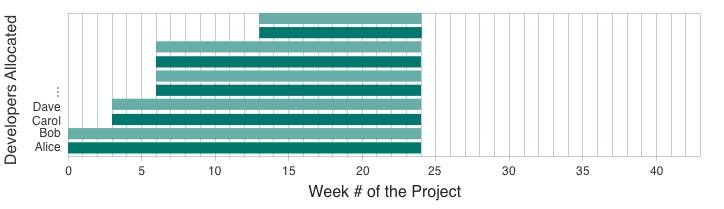
\includegraphics[width=7.1in]{OriginalDeveloperStaffingV2.jpg}
\caption{Planned Developer Staffing}
\label{PlannedDeveloperStaffing}
\end{figure*}

The 35-person project consisted of an iOS team of 10 engineers, an android team of 10 engineers, and a Java back-end team of 8 engineers with the support of 2 to 4 interaction designers and 3 product managers. For the purpose of this discussion, we will focus on the iOS team. 

The first iOS release to the Apple store occurred on week 23. Give the success of the project, the client extended the engagement for a second iOS release that occurred on week 43. 

On a typical project, the team is stable and organically grown. Figure \ref{PlannedDeveloperStaffing} shows the staffing plan at the start of Project Quattuor. Two developers started the project with additional developers rolling on as there were more tracks of work. The diagram shows when individual developers start and stop working on the project. 

On this project, developers were routinely rotated off and replaced for a variety of reasons, including being promoted to management, taking medical leave, leaving the company, transferring to a different office, transferring to another project, and taking vacations. 

The client wanted to maximize feature development regardless of cost. On a typical project, if an engineer goes on vacation, the team remains the same and is slightly less productive. On this project, someone took that person's place while the person was gone. This resulted in many engineers rolling on and off the project. A total of 22 people worked on the ten-person project. The ongoing rotation of team members likely undermined the team's sense of identity \cite{TuckmanModel}.

\begin{figure*}[t]
\centering
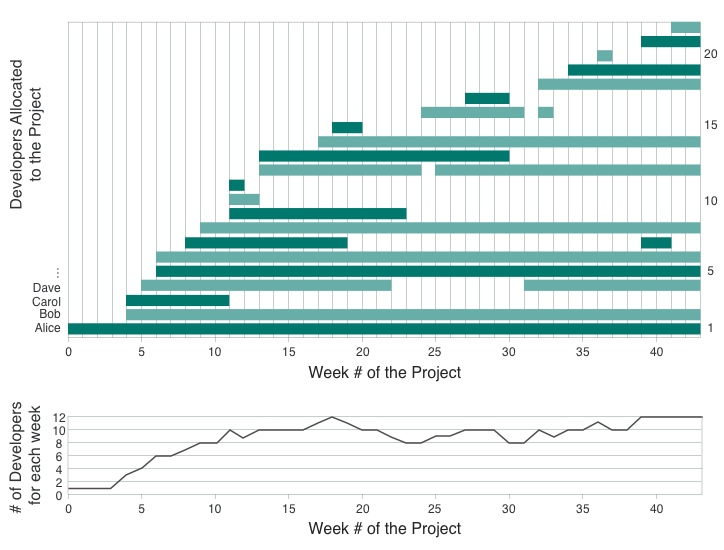
\includegraphics[width=7.1in]{DeveloperStaffingV4.jpg}
\caption{Actual Developer Staffing}
\label{DeveloperStaffing}
\end{figure*}

Figure \ref{DeveloperStaffing} shows the actual project staffing.  The bar chart on the figure's top part shows that there were five developers who were on the project for most of its duration, that 22 people actually worked on the project, and that the maximum team size was 12 developers working together at the same time.

The graph on the figure's bottom shows the total number of developers allocated to the project at any given week. There is a steady ramp up from week 5 to week 12. The average number of developers assigned to the team is 9.8 and the maximum team size was 12 developers.

The project experienced many challenges, including the unstable team, not having access to production back-end systems or expensive dependent physical components, and cultural differences between Pivotal and the client's deployment organization. Yet the team successfully completed the project. The client was delighted, even claiming with the first release that the team had delivered a multiple year project in 5 months. 

Conventional wisdom says that team disruption should be avoided. Yet, Project Quattuor succeeded despite high team churn. This observation leads us to our first research question: \quotes{How does Pivotal overcome team disruption in software development?}

\begin{table*}[t]
\renewcommand{\arraystretch}{1.5}
\centering
\caption{Theory of Sustainable Software Development: Principles, Policies, and Practices}
\label{SustainableSoftwareDevelopmentTable}
\begin{tabular}{|p{1.65in}|p{1.35in}|p{1.8in}|p{1.6in}|}
\hline
\multicolumn{4}{|c|}{Sustainable Software Development}                     \\
\hline
Underlying Principles & Policies                  & Removing Knowledge Silos Practices & Caretaking the Code Practices       \\
\hline
Keeping a Positive Attitude Toward Team Disruption & Team Code Ownership & Continuous Pair Programming         & TDD / BDD                   \\
Encouraging Knowledge Sharing and Continuity & Shared Schedule           & Overlapping Pair Rotation & Continuous Refactoring      \\
Caring about Code Quality  & Avoid Technical Debt      & Knowledge Pollination    & Supported by Live on Master \\ 
\hline
\end{tabular}
\end{table*}


\section{Theory of Sustainable Software Development}
\label{Theory}

A theory of Sustainable Software Development summarized in Table \ref{SustainableSoftwareDevelopmentTable} emerged from the grounded theory research. Sustainable Software Development is characterized by a collection of synergistic principles, policies, and practices. 

The primary concern of Sustainable Software Development is enabling any pair to be able to work on any story in the backlog. The principles encourage a positive attitude towards team disruption, knowledge sharing and continuity, as well as caring about code quality. The goal of any pair picking up any story is achieved by actively removing knowledge silos and caretaking the code. 

The theory answers the following research question:

Research Question: How does Pivotal overcome team disruption in software development?

Pivotal overcomes the challenge of team disruption through the set of principles, policies, and practices described in the following sections.
\subsection{Principles}

\subsubsection{Keeping a Positive Attitude Toward Team Disruption}
Conventional wisdom says that team disruption should be avoided. Yet, team disruption is a reality in the industry, as exemplified by Project Quattuor where only four of twenty-two developers worked on the project from beginning to end (see Figure \ref{DeveloperStaffing}.) However, the observed organization kept a positive attitude towards disruption, transforming a challenge into an opportunity and hence demonstrating remarkable business agility. Team members rolling off the project were replaced as needed. New members rolling onto the project were viewed as an opportunity to improve the current code base by providing a fresh, new perspective. When a new team member did not understand the code base, he or she revealed issues with code discoverability. New team members often questioned the team's assumptions and challenged \quotes{cargo culting.} 

The first underlying principle of Sustainable Software Development is keeping an open and positive attitude towards team disruption, transforming a challenge into an opportunity to improve code quality.

\subsubsection{Encouraging Knowledge Sharing and Continuity}
Despite the fresh perspectives added by new team members, team disruption could potentially result in significant knowledge loss for the organization. A set of policies and practices aiming at encouraging knowledge sharing and continuity mitigates this risk. These policies are Team Code Ownership and Shared Schedule, while the practices are Continuous Pair Programming, Overlapping Pair Rotation, and Knowledge Pollination. Refer to the following sections for more on these policies and practices. 

The second underlying principle of Sustainable Software Development is encouraging knowledge sharing and continuity, enabling the knowledge to spread from one developer to the next, and eventually reach the entire team. Knowledge sharing and continuity make the team more resistant to disruption. 

\subsubsection{Caring about Code Quality}

Enabling knowledge sharing and continuity does not guarantee sustainable development if the team starts incurring technical debt  \cite{McConnellTechnicalDebt}. A set of policy and practices aimed at taking good care of the code itself mitigates this risk. The policy is Avoid Technical Debt, while the practices are Test Driven Development / Behavior Driven Development and Continuous Refactoring. Refer to the following sections for more on these policy and practices.

The third underlying principle of Sustainable Software Development is caring about code quality, hence avoiding technical debt and enabling sustainable team productivity.

Table \ref{SustainableSoftwareDevelopmentTable} summarizes a set of policies and practices that implement the principles which are recorded in the following sections. For each practice, we present how it is used at Pivotal, and discuss anti-patterns and potential alternatives. We provide deeper descriptions for practices rarely documented in the literature.
\subsection{Policies}

\subsubsection{Team Code Ownership}

\textbf{Description:} Team code ownership conveys that any developer on the team can improve any part of the system at any time \cite{BeckExtremeProgramming2004}. 

\textbf{Purpose:} Everyone is responsible for the whole system. An organization saying, \quotes{Anyone can modify any piece the code} is not sufficient to achieve the desired result of team code ownership. Achieving team code ownership requires a set of enabling practices. These enabling practices aim at removing knowledge silos and taking good care of the code, as described in the following sections.

\textbf{At pivotal:} Every developer is empowered to work on any part of the system and is encouraged to refactor any code section to improve its quality as needed, especially when code discoverability and readability is an issue.

\textbf{Anti-pattern:} Removing team code ownership makes sustainable software development challenging. Every line of code written via strong ownership creates a knowledge silo. Code reviews are a mitigation strategy with an asynchronous delay. When the delay is too long, merging code onto the master becomes problematic, which then places pressure to avoid Continuous Refactoring.  

\subsubsection{Shared Schedule}
\textbf{Description:} Shared Schedule signifies that all project team members share the same work schedule. 

\textbf{Purpose:} Shared Schedule enables the Continuous Pair Programming, Overlapping Pair Rotation, and Knowledge Pollination practices. With Shared Schedule, teams form new pairs at the beginning of the day. The evening becomes a natural interruption to the continuous software development workflow. 

\textbf{At pivotal:} Team members at the Palo Alto office start working at 9:00 in the morning and leave at 5:00 in the evening, five days a week. This is done without management coercion; each team member agreed to this fixed schedule to achieve the benefits of Sustainable Software Development. When Shared Schedule is the normative, flexibility is possible for exceptions. For instance, seeing the doctor during the day is fine since it is important to take care of oneself.

Pivotal prefers for all team members to be co-located as it promotes synchronous and osmotic communication. As an exception, Project Quattuor was a two-office project with half the team members in Palo Alto and half the team members in San Francisco. The team utilized remote pairing each day for Knowledge Pollination. Future research could explore whether Sustained Software Development works for a distributed team with a Shared Schedule.

\textbf{Anti-pattern:} Flexible work hours potentially jeopardizes Continuous Pair Programming, Overlapping Pair Rotation, and Knowledge Pollination practices. A team with flexible work hours might find it difficult to pair program on all stories (as described in the Continuous Pair Programming practice.) A team member consistently soloing from 8:00 am to 10:00 am might be building knowledge silos. 

When developers arrive whenever they feel like it, rotating pairs (as described under the Overlapping Pair Rotation practice) becomes awkward, as there is no longer a natural time to rotate pairs. Trying to schedule a time midday to rotate pairs feels artificial. Even if the team says they will rotate later in the day, once pairs get into their stories and form context on what needs to be done, they typically forget about repairing until it is time to go home.

Pivotal experimented with pairing when developers arrived, but this meant that developers arriving early were making decisions for the team members who arrived later, hence loosing some benefits of pair programming. 

\textbf{Alternatives:} A possible mitigation strategy could be to adopt core work hours. Individuals would solo on simple cleanup chores outside of core hours, and switch to pair programming for feature development when the whole team is in the office.  

\subsubsection{Avoid Technical Debt}
\textbf{Description:} Technical Debt refers to delaying needed technical work, by taking technical shortcuts, usually in pursuit of calendar-driven software schedules \cite{McConnellTechnicalDebt}.  

\textbf{Purpose:} Avoid Technical Debt enables a team to balance feature development with Continuous Refactoring (as described under the Continuous Refactoring practice.) When a team is pressured to finish work by a deadline, they might be tempted to focus on feature delivery, take on technical debt, and stop refactoring. When a team delays refactoring and takes on technical debt, the code becomes harder to work with, which in turn makes it harder for developers to rotate onto that part of the code base. There is a dialectic tension \cite{RalphProcessTheories} between Continuous Refactoring and delivering more features while accruing technical debt.

\textbf{At pivotal:} When a team implements a feature, the team endeavors to build it well. A pair tends to create well-crafted code by avoiding shortcuts and short-term fixes. Even with changing features or a changing product vision, the team strives to have well-engineered code. The team codes for the \quotes{present} by building the simplest solution for the current story. The team eschews over-engineering for potential future features. The team avoids technical debt by building the best solution for the moment at hand.  

\textbf{Anti-pattern:} On Project Quattuor, the product manager suggested that the team deliver more stories at the cost of technical debt to make a release date. Some team members followed this suggestion, skipped the refactoring step, and introduced harder to maintain code. This decision made it difficult for pairs to rotate onto parts of the code. Pairs making the decision to skip refactoring caused future pain for the next pair to work with that part of the code. Immediately after the first release, the team spent several weeks refactoring the code to pay down the debt and be able to consistently deliver new features again. During stressful times it is critical for the team to double down on its practices and be more disciplined.
\subsection{Removing Knowledge Silos Practices}
This section presents practices for encouraging knowledge sharing and continuity, enabling the knowledge to spread from one developer to the next, and eventually reach the entire team, as illustrated in Figure 3, where letters A to F represent 6 developers working in pairs.

\begin{figure}[t]
\centering
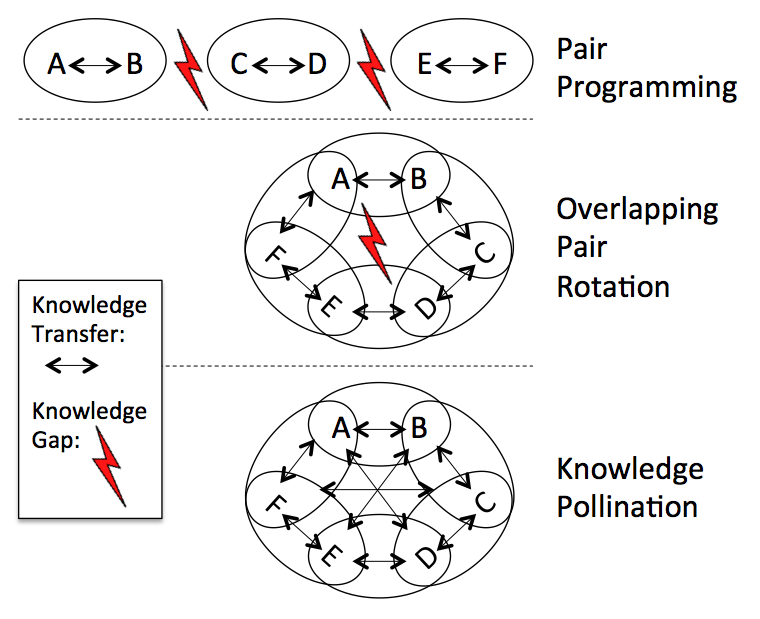
\includegraphics[width=3.4in]{KnowledgeSharingLevels.png}
\caption{Three Levels of Knowledge Sharing}
\label{KnowledgeSharing}
\end{figure}

\subsubsection{Continuous Pair Programming}
%what
\textbf{Description:} Continuous Pair Programming is two developers collaborating to write software together as their normal mode of software development.

%why
\textbf{Purpose:} When two developers work together, they are likely to bring more knowledge, and generate more diverse solutions compared to a solo developer. Having two pairs of eyes increases the potential of catching defects. When two developers work together, knowledge spreads from one developer to the next, as illustrated in Figure 3. Overall, pairing reduces knowledge silos and can improve code quality.

%at pivotal
\textbf{At pivotal:} Pairing happens with two monitors, two keyboards, two mice, and one computer. Developers always work in pairs, unless exceptional circumstances arise. For instance, solo programming occurs when one developer is out of the office for part of the day (e.g. at home to let a plumber in, or at the doctor's office) or out of the office the whole day (e.g. out sick) or involved in another business activity for a few hours (e.g. interviewing candidates, scoping a new project.) When solo programming, developers take low-risk chores, refactorings, or stories. With any sizable project, there usually is something the team has been meaning to do that one person can safely do and report back to the team on its completion.  

%removing
\textbf{Anti-pattern:} Removing this practice results in solo programming where there is a clear owner for the code written. This would increase individual ownership and start creating knowledge silos. 

%alternatives
\textbf{Alternatives:}  In solo programming, to remove silos, developers could take the stories for the part of the code they know least about. Assigning stories to developers who have the least understanding of the code could be a hard sell to management as it slows productivity down (at least initially.) Bird's study \cite{BirdDontTouchMyCode} suggests that this approach would introduce more defects. 

\subsubsection{Overlapping Pair Rotation}
\textbf{Description:} Overlapping Pair Rotation happens when there is a daily rotation of the people working on a track of work: one developer rolls off and another developer rolls on. This results in knowledge continuity for a track of work, as illustrated in Figure 3. Typically, rotations happen in the morning as the evenings provide a natural interruption to work. 

\textbf{Purpose:} The rotation of developers helps spread knowledge and promotes team code ownership. The goal is to prevent the situation where one developer must be on the story since only that person understands how that part of the system works. The entire team should be able to modify the code. Rotation helps prevent knowledge silos and individual code ownership from forming. 

\textbf{At pivotal:} Whenever a knowledge silo begins to emerge, the team actively fights against it and tries to spread that knowledge around through pair rotation.  Currently, there are three strategies in use. 

\textit{Optimizing for people rotation:} Most teams rotate based on who has paired with whom. Developers try to pair with the person they \quotes{least recently paired with} (basically a Least Recently Used strategy.) Some teams use rotation techniques or tools to track this information.

As a downside, the strategy does not clearly articulate the purpose of knowledge silo removal and the need for knowledge transfer. As an example, developers who recently left a track of work might ask to be rotated back without realizing the potential cost to the team. This prevents an opportunity to spread the knowledge to the rest of the team. (On a four person team, this is not an issue.)

\textit{Optimizing for individual preferences:} A few teams allow developers to pick with whom they will work or on which stories to work based on individual preferences. This has the same downsides as the previous strategy. 

\textit{Optimizing for context sharing:} A few teams are experimenting with rotating onto a track the person who has not been working on the track for the longest time. The goal each day is for the developer leaving the track next to empower the developer whom will remain on the track. Before any rotation, the remaining developer is asked, \quotes{Was enough context shared with you?} If the answer is no, then the first developer does not leave and the pair continues to work together for another day. This provides a feedback loop on how well the team is transferring knowledge. 

\textbf{Anti-pattern:} Removing this practice means that developers can work on the same part of the code base for extended periods of time, developing individual code ownership and knowledge silos. One interviewee described their experience at a previous company that follows Extreme Programming. Developers could be paired for more than a month working on only one part of the system. This lack of pair rotation led to building deep knowledge silos. 

Ideally developers work on the next, non-blocked story at the top of the backlog. When developers start skipping down the backlog, it can be an indication that they might not have enough context to work on any story. On Project Quattro, there was a knowledge silo with a complex bug related to an obsolete technology that only a handful of people understood. Often developers would skip over stories and bugs related to that technology. At one point, the product manager reminded the team to keep \quotes{working from the top of backlog.}

Sometimes a developer wants to see a story through to completion over multiple days. Maybe he or she loves the technology or the feature. In these situations, the team needs to be careful about forming knowledge silos and creating a sense of personal ownership.

If the team says \quotes{We need Marion on that story, only she really knows the Apple watch code base,} or \quotes{Shea knows the ins-and-outs of the legacy integration, we need him to work on this story,} then these are signs that knowledge silos have emerged. 

\textbf{Alternatives:} Team members that build a knowledge silo can share what they learned through a demo, code walk through, or a team huddle. This helps a team share knowledge, but is less effective than working directly with the code. 

\subsubsection{Knowledge Pollination}
\textbf{Description:} Knowledge Pollination refers to the set of activities contributing to knowledge sharing in an unstructured way. Examples include daily stand-up meetings, writing or sketching on whiteboards, overhearing a conversation, using the backlog to communicate current status about a story, calling out an update to the entire team, or simply reaching out to others to ask questions as needed. 

\textbf{Purpose:} Knowledge Pollination contributes to spreading knowledge among the team as illustrated in Figure 3.

\textbf{At pivotal:} Daily standups create awareness of who is working on what. Teams can write down a \quotes{parking lot} of issues to discuss during daily standups. A pair may record the current status of a blocked story so that the next pair picking it up knows the situation. Osmotic communication helps when the person who worked on a story overhears another pair discussing a class for instance.

Calling out an update to the entire team might be a simple as shouting \quotes{The build is broken, we are looking into it}, or this interchange:  \quotes{We just checked in a presenter} followed by \quotes{We just used your presenter. That's great collaboration.}

While working on a story, a pair may discover that they are missing some key context that prevents them from efficiently proceeding. If the issue is about the acceptance criteria for a story, they clarify with the product manager. If the issue is about the code base, the pair can ask the people who recently worked on that section of code, or ask the entire team.  To determine whom to ask, the pair may remember who did what at stand-up, look through tracker to see who worked on a story, or check out source code version history (e.g. git annotate.) Two-, four-, and six- person teams tend to have collective memory of who worked on which features from daily standup. A ten-person team might need to be active in finding the answer to the question. 

Instead of thrashing, a pair interrupts another pair to gain the needed information. Thus, interruptions are encouraged as they make the entire team more efficient as knowledge pollinates across the team. 

These mechanisms help a team build awareness. Chong observed that \quotes{transmission of awareness information is a relatively effortless act in the XP environment} in her ethnographic study of an Extreme Programming team compared to a traditional team \cite{ChongNominum}.
 
\textbf{Anti-pattern:} An organization that provides little opportunity to share knowledge leads to wasted time as developers must acquire the knowledge through other means or end up reinventing the wheel.
\subsection{Caretaking the Code Practices}
\subsubsection{Test Driven Development, Behavior Driven Development}
\textbf{Description:} In Test Driven Development (TDD) developers write unit tests before creating a design and writing code. In Behavior Driven Development (BDD) developers implement acceptance tests before creating a design and writing code. Most lines of production code are tested before the production code is written. The software's design emerges from the tests and subsequent refactorings.

In Extreme Programming Kent Beck describes his corresponding \quotes{Testing} practice as developers writing \quotes{automated unit tests} and implementing customer provided \quotes{functional tests} for story acceptance \cite{BeckExtremeProgramming2000}. Later, Kent Beck refines these ideas as \quotes{Test-first programming} \cite{BeckExtremeProgramming2004}. 

\textbf{Purpose:} This practice creates a safety net and empowers a pair to have the confidence to modify the code base. This enables any pair to pick up any story. Continuous Refactoring results in easier to modify tests.

\textbf{At Pivotal:} Developers use a combination of TDD and BDD. While each project is different, programmers tend to use BDD to describe interactions between the user and the system and TDD at a unit test level. Teams use a variety of TDD strategies including testing the responsibilities and interactions \cite{Goose} or contract testing using mocks as described by J. B. Rainsberger \cite{RainsbergerIntegrationTestsYouTube}. In Pivotal's ideal, the design emerges from the creation and exploration of the test cases.  

\textbf{Anti-pattern:} Removing this testing practice means that developers no longer have the confidence to change any part of the code as they may unknowingly end-up breaking something else. 

\textbf{Alternatives:} For a system without a test suite documenting the system specification, a possible remedy is creating knowledge silos where developers own particular parts of the system and understand the ramifications of changes. Creating strong code ownership is exactly the problem that sustainable software development is trying to solve.

Writing tests after the code is written could produce a safety net for refactoring, provided that tests correctly exercise the system. (A test that was never red might not be testing anything.) We did not observe this behavior and future research is necessary to determine if any testing approach is sufficient for sustainable software development.

\subsubsection{Continuous Refactoring}
\textbf{Description:} Continuous Refactoring is the systematic improvement of the code base while feature work is being performed. When developers identify something wrong such as a code smell, they simply fix it. In this regard, developers are caretaking the code by continuously improving it. This practice results in an emergent software design, as well as empathy for the code as developers learn to \quotes{listen to the code.} 

%Continuous Refactoring is one way to prevent technical debt from accumulating. When a team employs continuous refactoring, the team refines a code base towards simple design, intention revealing code, and discoverable code. 

\textbf{Purpose:} Continuous Refactoring enables any pair to work on any part of the system. Taking the time to increase code discoverability, code readability, code modifiability, and code simplicity produces long-term benefits for the team. 

\textbf{At Pivotal:} Developers typically do some refactoring while implementing stories. Developers are encouraged to improve the code's design, make the code easier to understand, and increase the discoverability of a component based upon its responsibility. Usually, team prefers \quotes{pre-factoring} where the developer does the complicated work to make the implementation of the current story as simple and easy as possible, as opposed to \quotes{post-factoring} where refactoring happens after the story is done, but before it is delivered.  

\textbf{Anti-pattern:} Removing this practice might produce hard to modify and messy code. Developers might not be able to easily work on any part of the code base. When refactoring is skipped, code might be simply bolted on to the existing design. Soon it becomes increasingly difficult to bolt more code on. A dilemma arises for the programmers working on the next story: do they continue bolting on more code, or do they perform the pretermitted refactorings. Removing this practice may also result in hard-to-change tests.

\textbf{Alternatives:} There are extreme situations where postponing refactoring for later becomes necessary. For instance, when the company might go out of business unless the company releases the next version. These moments should be considered carefully. The team risks taking on uncontrolled technical debt as \quotes{refactoring later} turns into \quotes{refactoring never.} 

\subsubsection{Live on Master}
\textbf{Description:} Live on master means that developers integrate their code several times a day, as quickly as possible. ExtremeProgramming.org calls this practice \quotes{Integrate Often.} \cite{IntegrateOften} 

\textbf{Purpose:} For teams to continuously refactor and minimize the waste of merge conflicts, the entire team needs to be routinely merging their code onto master.  If a pair communicates to the team that they are actively \quotes{refactoring} a component, they are asserting exclusive temporary ownership over the file to avoid merge conflicts. While this is a normal practice for a few hours, if it happens for multiple days, the team is losing collective ownership of that code. The team is not able to receive any of the benefits until the work is merged back to master. 

\textbf{At Pivotal:} In the ideal workflow, developers will merge their code to master many times a day. If a pair has not merged to master by the afternoon, the pair typically starts examining why this is difficult and explores ways of incrementally making changes. Developers may use branches to save spikes. When rotating pairs, developers may use branches to move work-in-progress code between machines.  

\textbf{Anti-pattern:} Removing this practice means that code lives in branches for days or weeks. Integrations might be painful due to merge conflicts and developers might delay needed refactorings. If a developer has code only on their machine, then no one else on the team can use or modify that code. When code lives only on one machine for many days in a row, the machine acts as a \quotes{virtual branch.} Running a Continuous Integration box and having long running branches is an anti-pattern.
\section{Theory Evaluation}
\label{TheoryEvaluation}

In assessing a Grounded Theory research study, Charmaz identifies four criteria for evaluating the theory: credibility (\quotes{Is there sufficient data to merit claims?}), originality (\quotes{Do the categories offer new insights?}), resonance (\quotes{Does the theory make sense to participants?}), and usefulness (\quotes{Does the theory offer useful interpretations?}) \cite{StolGTinSE}. 

\begin{itemize}
\item 
\textbf{credibility:}  The current data set is rich and lead to theory saturation. (Saturation means that the properties of the theory are complete and are not affected by new data.) The data set comprises 21 intensive interviews conducted in four different offices,  field notes from participant observation on Project Quattuor, and the primary researcher's involvement in four other projects as participant-observer.

\item
\textbf{originality:} The theory uniquely depicts the principles, policies, and practices enabling software development sustainability in an organization. Since the organization under study follows Extreme Programming, it is not surprising that many of the practices of Sustainable Software Development are defined in Extreme Programming. However, pair rotation and its supporting principles, policies, and practices are central and unique to the proposed theory.

\item
\textbf{resonance:} More work needs to be done to claim that the theory resonates with participants. So far, the theory has only been presented to a few participants, for whom the theory made perfect sense as it reflects the way they work. 

\item
\textbf{usefulness:}  The theory informs Pivotal engineers as to why Pivotal purposefully avoids knowledge silos, and how the theory's principles, policies, and practices work together to accomplish the team's goals.  The theory explains why the principles, policies, and practices should be incorporated together without taylorization. One engineering manager uses the theory to help potential clients understand how Pivotal achieves the business goals of both the client and Pivotal.

\end{itemize}

\section{Threats to Validity}

\subsection{External Validity}

\textbf{Generalizability across situations:} There are four broad types of scientific generalization: 1) from data to descriptions, 2) from descriptions to concepts, 3) from concepts to theory, 4) from theory to description \cite{Lee2003generalizing}. Grounded theory research involves the first three kinds of generalization. By contrast, in the constructivist epistemology adopted here, generalizing from a theory confirmed in one context to descriptions of a new context is done by the researchers in the new context, on a case-by-case basis. Grounded theory does not support statistical generalization from a sample to a population.

\subsection{Internal Validity}
\textbf{Researcher bias:} A risk of the participant-observer technique is that the researcher may lose perspective and become biased by being a member of the team. An outside observer might see something the researcher missed. We mitigated this risk by recording interviews and with a colleague reviewing the coding process.

\textbf{Prior knowledge bias:} With grounded theory, prior knowledge can aid the researcher in looking at interesting research questions or create difficulties by blinding the researcher about possible explanations \cite{GlaserIssues}. We mitigated this risk with a colleague reviewing the coding process. 
\section{Future Research}
Future research is necessary to validate the theory, especially when it comes to resonance and usefulness. Our plan is to present the theory to all study participants to understand their perspectives on both dimensions. 

In addition, we are interested in the tension between individual and team ownership, as well as the factors that foster and decrease the sense of ownership. Developers, interaction designers, and product managers all have different goals for their role. In future work, we plan to examine how the sense of ownership is driven by different factors for each role.

Some programmers naturally adapt to team code ownership, while others struggle with the transition. In future research we will follow new Pivotal engineers and examine their journey in transitioning from individual code ownership to team code ownership. Perhaps there are 
specific practices that Pivotal or the development team could employ to ease the transition. We will also investigate the optimal team size for team code ownership. 

\section{Conclusions}
This paper introduces the theory of \quotes{Sustainable Software Development} as a solution to the challenge of software development sustainability for an ever changing workforce. The theory emerged from a constructivist grounded theory research study. The study answers the research  question \quotes{How does Pivotal overcome team disruption in software development?} by collecting data from 21 intensive interviews conducted in four different Pivotal offices, field notes from participant-observation on the Project Quattuor, and the primary researcher's involvement in four other Pivotal projects as participant-observer.

The emergent theory is characterized by a collection of synergistic principles, policies, and practices encouraging a positive attitude towards team disruption, knowledge sharing and continuity, as well as caring about code quality. The theory refines and extends the understanding of Extreme Programming by adding a few principles, policies, and practices (like the unique Overlapping Pair Rotation practice) and aligning these principles, policies, and practices towards the business goal of sustainability.

Conventional wisdom says that team disruptions should be avoided, and that extensive documentation is needed to prevent knowledge loss during team churn. Unfortunately, documentation often quickly becomes unwieldy and unreliable, making this approach suboptimal. The theory positions team code ownership with overlapping pair rotation and knowledge pollination as an alternative and potentially more effective strategy to mitigate against knowledge loss.

The primary benefit to the employer is business agility. The engineering team continues to deliver software week after week, month after month, while surviving cataclysmic events. Things do not fall apart when the superstar developer leaves. People can go on vacation whenever they need to because features or components are not critically tied to a particular individual. The team leverages the whole team's talents. This removes bottlenecks of, \quotes{Only Pat can work on these features.} Critical feature work can be parallelized since anyone can work on the feature, as opposed to an individual code owner. 

The primary benefits to the engineer are the ability to understand the entire system, to work on every story, an increase in teaching opportunities to share one's expertise, and in-depth opportunities to learn the subtle parts of the technologies. 

%The primary cost is a shift from individual code ownership to team code ownership. For some engineers, their sense of value and self-worth is derived from direct code ownership, and thus transitions to Sustainable Software Development should not be taken lightly. Sustainable Software Development works well with collaborative individuals and may not be suited for people who like to work on their own. Sustainable Software Development works when team members have the maturity to hold temporary personal contributions loosely, understanding that the team may enhance any aspect of the product.

Sustainable Software Development is suited for companies that must routinely deliver value to their users, customers or stakeholders. Some companies are better positioned to withstand a quarter where nothing happens (from an external perspective) or  \quotes{The forgotten two years of management waste} as described by one manager in this study. Hopefully, competitors have not caught up or surpassed the organization during the lost time. Both Pivotal Labs as a consulting practice and the growth of Pivotal's Cloud Foundry towards market dominance depend on the continual development of features. Neither can afford to falter, and both implement Sustainable Software Development. Sustainable Software Development enables software development to continue at a regular pace regardless of who is on the team, or rather, regardless of changes in team composition.

\section{Acknowledgement}

Thank you to Rob Mee, David Goudreau, Ryan Richard, and Zach Larson for making this research possible. Thank you to Karina Sils for creating Figure \ref{PlannedDeveloperStaffing} and Figure \ref{DeveloperStaffing} using Sketch.





% \begin{table*}[t]
% \renewcommand{\arraystretch}{1.3}
% \centering
% \caption{Sustainable Software Development of software development}
% \label{Practicesl}
% \begin{tabular}{p{1.1in}p{5.0in}}
% \hline
% purpose            & business sustainability for evolving workforce. This enables a way of working that allows the product to continue evolving while workforce is changing by cross-sharing knowledge and simplifying code so that it is easy to maintain \\ 
% \hline
% mechanism          & shares decision making power on the entire code base for accomplishing a common goal. For each feature, many developers shape the implementation  \\ 
% \hline
% enabling practices & 1. Collective code ownership      \\ 
%                   & 2. Continuous refactorings and sustainable work pace                     \\ 
%                   & 3. Pair programming                                    \\ 
%                   & 4. Rotating developers when context shared    \\ 
%                   & 5. Test Driven Development, Behavior Driven Development     \\ 
%                   & 6. Live on Master                 \\ 
%                   & 7. Obtaining context  \\ 
% \hline
% benefits           & Team Benefits                                                                                                                                                                                  \\ 
%                   & - permeates knowledge across the whole team; increasing the amount of shared knowledge and context                                                                                               \\ 
%                   & - leverages whole team's talents                                                                                                                                                                 \\ 
%                   & - enables and empowers any pair to change any part of code (authority and responsibility)                                                                                                        \\ 
%                   & - anyone can work on anything                                                                                                                                                                    \\ 
%                   & - enables seamless transitions of rotating people on to and off a project                                                                                                                        \\ 
%                   & Product Benefits                                                                                                                                                                               \\ 
%                   & - routine defect detection by many developers reading and augmenting the code                                                                                                                    \\ 
%                   & Code Benefits                                                                                                                                                                                  \\ 
%                   & - increasing discoverability (knowing which class is responsible for something)                                                                                                                  \\ 
%                   & - separating concerns                                                                                                                                                                            \\ 
%                   & - simplifying control flow                                                                                                                                                                       \\ 
%                   & - increasing design consistency                                                                                                                                                                  \\ 
%                   & - increasing flexibility (pliable code allowing more refactorings)                                                                                                                               \\ 
%                   & - increasing readability (understanding how a method works)                                                                                                                                      \\ 
% \hline
% risks              & large team sizes means that it is hard for the team to have shared context as so much parallel work is being done which decreases empowerment                                                  \\ 
%                   & thinking that someone else will improve codebase which means team is not reducing technical debt and increasing code apathy                                                                    \\ 
%                   & naively modifying code without understanding context and severity of changes which introduces defects                                                                                          \\ 
%                   & artificial team stress can affect business sustainability as the team takes on technical debt that decreases sense of ownership                                                                \\ 
%                   & knowledge silos need to be spread amongst the team                                                                                                                                             \\ 
% \hline
% costs              & May be less efficient when two people might work on something simple                                                                                                                           \\ 
%                   & For some individuals, personal ownership might be larger motivator than communal ownership. In these cases, personal ownership may have higher short-term productivity                         \\ 
%                   & Flexible work hours benefit, cherished by many, make business sustainability challenging to implement. Effective pairing and context sharing requires a consistent synchronized schedule       \\ 
% \hline
% indicators that you are doing it wrong   & emerging knowledge silos \\                                                                                                                                                                                                                                   
% \hline
% \end{tabular}
% \end{table*}








% The following two commands are all you need in the
% initial runs of your .tex file to
% produce the bibliography for the citations in your paper.
\bibliographystyle{abbrv}
\bibliography{bibliography}  % sigproc.bib is the name of the Bibliography in this case
% You must have a proper ".bib" file
%  and remember to run:
% latex bibtex latex latex
% to resolve all references
%
% ACM needs 'a single self-contained file'!
%

% That's all folks!
\end{document}
